\documentclass[10pt,twocolumn,letterpaper]{article}

\usepackage{cvpr}
\usepackage{times}
\usepackage{epsfig}
\usepackage{graphicx}
\usepackage{amsmath}
\usepackage{amssymb}

\def\cvprPaperID{1} % *** Enter the CVPR Paper ID here

\usepackage[breaklinks=true,bookmarks=false]{hyperref}

\cvprfinalcopy % Comment this line and it stop working! :(
\ifcvprfinal\pagestyle{empty}\fi

\def\httilde{\mbox{\tt\raisebox{-.5ex}{\symbol{126}}}}

% Pages are numbered in submission mode, and unnumbered in camera-ready
%\ifcvprfinal\pagestyle{empty}\fi
\setcounter{page}{1}

\graphicspath{ {./images/} } 

\sloppy

%-------------------------------------------------------------------------
%-------------------------------------------------------------------------

\begin{document}

%%%%%%%%% TITLE
\title{\textit{Project Milestone:} Convolutional Neural Network to Image Segmentation}

\author{Felipe Augusto Lima Reis\\
PUC Minas - Pontif\'icia Universidade Cat\'olica de Minas Gerais\\
R. Walter Ianni 255 - Bloco L - Belo Horizonte, MG, Brasil\\
{\tt\small falreis@sga.pucminas.br}
}

\maketitle
%\thispagestyle{empty}

%%%%%%%%% ABSTRACT
\begin{abstract}
   The ABSTRACT is to be in fully-justified italicized text, at the top
   of the left-hand column, below the author and affiliation
   information. Use the word ``Abstract'' as the title, in 12-point
   Times, boldface type, centered relative to the column, initially
   capitalized. The abstract is to be in 10-point, single-spaced type.
   Leave two blank lines after the Abstract, then begin the main text.
   Look at previous CVPR abstracts to get a feel for style and length.
\end{abstract}

%%%%%%%%% BODY TEXT
\section{Introduction} \label{introduction}

Image segmentation refers to the partition of an image into a set of regions to cover it, to represent meaningful areas \cite{DOMINGUEZ}. The goal is to simplify and/or change the representation of an image into something
that is more meaningful and easier to analyze \cite{AHMED_SARMA}.

Segmentation has two main objectives: the first one is to decompose the image into parts for further analysis and the second one is to perform a change of representation \cite{DOMINGUEZ}. Also, segmentation must follow some characteristics to identify regions, as it follows:

\begin{itemize}
 \item Regions of an image segmentation should be uniform and homogeneous with respect to some characteristic, such as gray level, color, or texture \cite{DOMINGUEZ};
 \item Region interiors should be simple and without many small holes \cite{DOMINGUEZ};
 \item Adjacent regions of a segmentation should have significantly different values with respect to the characteristic on which they are uniform \cite{DOMINGUEZ};
 \item Boundaries of each segment should be smooth, not ragged, and should be spatially accurate \cite{DOMINGUEZ}.
\end{itemize}

The future paper will evaluate segmentation methods using Deep Neural Networks and compares with classical methods of segmentation, using the superpixels approach. Also, the paper will evaluate the composition of classical methods with DNN approach, to speed up the training process and become more accurate.

The organization of this paper is as follows. In the next Section we discuss the problem statement. In Section \ref{sec:tech_approach} its explained how the will work and the results we expect. Then in Section \ref{sec:results} we present an some preliminary results.

%-------------------------------------------------------------------------
\section{Problem Statement} \label{sec:prob_statement}

The future paper will evaluate segmentation methods using Deep Neural Networks and compares with classical methods of segmentation, using the superpixels approach. Also, the paper will evaluate the composition of classical methods with DNN approach, to speed up the training process and become more accurate.

To provide the goals we explained in Section \ref{introduction}, the paper will use Convolutional Neural Networks provided by the literature. To provide segmentation the paper will use SEGNET, a deep encoder-decoder architecture for multi-class pixelwise segmentation \cite{SEGNET}. 

The SEGNET architecture consists of a sequence of non-linear processing layers (encoders) and a corresponding set of decoders followed by a pixelwise classifier \cite{SEGNET} \cite{SEGNET_WEBSITE}. Typically, each encoder consists of one or more convolutional layers with batch normalisation and a ReLU non-linearity, followed by non-overlapping maxpooling and sub-sampling \cite{SEGNET} \cite{SEGNET_WEBSITE}. The sparse encoding due to the pooling process is upsampled in the decoder using the maxpooling indices in the encoding sequence \cite{SEGNET} \cite{SEGNET_WEBSITE}. Figure \ref{fig:segnet} presents the architecture of SEGNET.

\begin{figure}[ht]
  \centering
  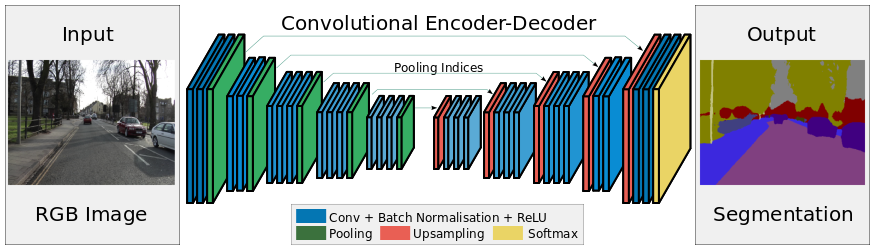
\includegraphics[width=0.48\textwidth]{segnet.png}
  \caption{SEGNET architecture. \textit{Image adapted from SEGNET project website} \cite{SEGNET_WEBSITE} \cite{SEGNET}}
  \label{fig:segnet}
\end{figure}

\cite{VGGNET} \cite{UNET}.

Main Dataset: Berkeley Segmentation Data Set and Benchmarks 500 (BSDS500)
○ Provides Contour Detection and Image Segmentation Resources;
○ As BSDS500 provides few images, it will be necessary using Data Augmentation;
○ Other possible datasets: KITTI Road
Evaluation: BSDS500 Performance Evaluation
○ Provides evaluation using Precision and Recall Method;
○ Code in Matlab provided with BSDS500 dataset \cite{BSDS500}.

%-------------------------------------------------------------------------
\section{Technical Approach} \label{sec:tech_approach}

%-------------------------------------------------------------------------
\section{Preliminary Results} \label{sec:results}

%-------------------------------------------------------------------------

{\small
\bibliographystyle{ieee}
\bibliography{egbib}
}

\end{document}
